Before the whole conception of the system, a general conceptual architecture of the system should be defined initially. In order to help understanding how the system works, the primary data flow between different domains will also be described.

\subsection{Architecture} \label{Architecture}
According to the analysis result of Single-Page-App in chapter 3, and considering the demand on high interactivity and ubiquity as well as scalability in the graphical discuss system, leveraging SPA architecture will benefit a lot and accelerate the implementation of the system. 

In general, the entire system will be divided into two parts: namely client and server-side. Each side is basically full independent to the other and has its own responsibility. 

\begin{enumerate}
\item
\textbf{Client}: The client is totally responsible for template rendering and view re-render as the view model changes. 
\item
\textbf{Server}: The server is in charge of core business logic, data processing, data persistence and also provides the client interfaces for data acquisition.
\end{enumerate}

% General Architecture of System including Server(data persistence with db) + Client(has multiple views, one template engine, re-render with new data.)
\begin{figure}[!htbp]
  \caption{placeholder}
  \centering
    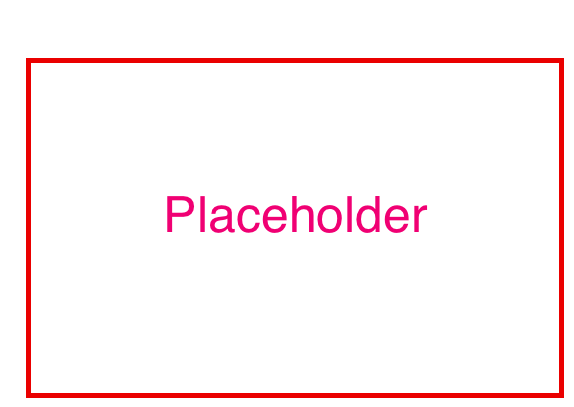
\includegraphics[width=0.6\textwidth]{Figures/placeholder.png}
  \label{fig:placeholder}
\end{figure}

General architecture of the system is described in figure XXX, the only bridge between the client and server-side is data transmission service. Complete separation of both sides will also accelerate the development flow in implementation phase. Once the protocol of data transmission services is fully confirmed and defined, development of each side is able to performed parallelly. Furthermore, technical choices on both sides are more flexible. Both sides are able to apply the technologies which fit them most without coupling to each other, the only thing they should obey is to follow the protocol of data transmission.

\subsection{Communication}
As mentioned above in \ref{Architecture}, data communication is the only coupling factor in the general architecture.

% restful - non-realtime

% websocket - Realtime
% Pic broadcast to multiple clients with different events. engine to rerender
